\fenicschapter{FFC: the FEniCS form compiler}
              {FFC: the FEniCS form compiler}
              {Anders Logg, Kristian B. \O{}lgaard, Marie E. Rognes and Garth N. Wells}
              {logg-1}

\index{FFC}
\index{form compiler}

One of the key features of FEniCS is automated code generation for
the general and efficient solution of finite element variational
problems. This automated code generation relies on a form compiler for
offline or just-in-time compilation of code for individual forms. Two
different form compilers are available as part of FEniCS. This chapter
describes the form compiler FFC. The other form compiler, SFC, is
described in Chapter~\ref{chap:alnes-3}.

\index{SFC}

%------------------------------------------------------------------------------
\section{Compilation of variational forms}

In simple terms, the solution of finite element variational problems
is based on two ingredients: the assembly of linear or nonlinear
systems of equations and the solution of those equations. As a result,
many finite element codes are similar in their design and
implementation. In particular, a central part of most finite element
codes is the assembly of sparse matrices from finite element bilinear
forms. In Chapter~\ref{chap:logg-3}, we saw that one may formulate a
general algorithm for assembly of sparse tensors from variational
forms. However, this algorithm relies on the computation of the
element tensor~$A_T$ as well as the local-to-global mapping~$\iota_T$.
Both $A_T$ and $\iota_T$ differ greatly between different finite
elements and different variational forms. Special-purpose code is
therefore needed. As a consequence, the code for computing $A_T$ and
$\iota_T$ must normally be developed by hand for a given
application. This is both tedious and error-prone.

\index{element tensor}
\index{local-to-global mapping}

The issue of having to develop code for $A_T$ and $\iota_T$ by hand
can be resolved by a form compiler. A form compiler generates code for
computing $A_T$ and $\iota_T$. This code may then be called by a
general purpose routine for assembly of finite element matrices and
vectors. In addition to reduced development time, performance may be
improved by using code generation since the form compiler can generate
efficient code for the computation of $A_T$ by using optimization
techniques that are not readily applicable if the code is developed by
hand. In Chapters~\ref{chap:oelgaard-2}, \ref{chap:kirby-8}
and~\ref{chap:kirby-4}, two different approaches to the optimized
computation of the element tensor~$A_T$ are presented.

From an input describing a finite element variational problem in
mathematical notation, the form compiler FFC generates code for the
efficient computation of $A_T$ and $\iota_T$, as well as code for
computing related quantities. More specifically, FFC takes as input a
variational form specified in the UFL form language (described in
Chapter~\ref{chap:alnes-1}) and generates as output C++ code that
conforms to the UFC interface (described in
Chapter~\ref{chap:alnes-2}). This process is illustrated schematically
in Figure~\ref{fig:logg-1:formcompiler}.

\begin{figure}
  \begin{center}
    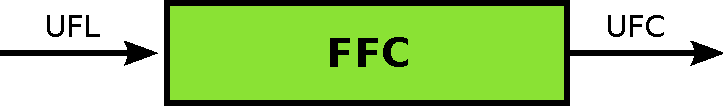
\includegraphics[width=10cm]{chapters/logg-1/pdf/ufl_ffc_ufc.pdf}
    \caption{The form compiler FFC generates C++ code in UFC format
      from a given finite element variational form in UFL format.}
    \label{fig:logg-1:formcompiler}
  \end{center}
\end{figure}

%------------------------------------------------------------------------------
\section{Compiler interfaces}

FFC provides three different interfaces: a Python interface,
a command-line interface, and a just-in-time (JIT) compilation
interface. The first two are presented here, while the third is discussed
below in Section~\ref{sec:logg-1:jit}. Although FFC provides three
different interfaces, many users are never confronted with any of these
interfaces; Python users mostly rely on DOLFIN to handle the communication
with FFC. The command-line interface is familiar for DOLFIN C++ users,
who must call FFC on the command-line to generate code for inclusion in
their C++ programs. The JIT interface is rarely called directly by users,
but it is the main interface between DOLFIN and FFC, which allows DOLFIN
to seamlessly generate and compile code when running solver scripts
implemented in Python.

%------------------------------------------------------------------------------
\subsection{Python interface}

The Python interface to \ffc{} takes the form of a standard
Python module. There are two main entry point functions to the
functionality of \ffc{}: \emp{compile\_form} and
\emp{compile\_element}, to compile forms and elements, respectively.

\index{\emp{compile\_form}}
The \emp{compile\_form} function provides the main functionality of
FFC, which is to generate code for assembly of matrices and vectors
(tensors) from finite element variational
forms. The \emp{compile\_form} function expects a form or a list of
forms as input along with a set of optional arguments:
%
\begin{python}
compile_form(forms,
             object_names={},
             prefix="Form",
             parameters=default_parameters())
\end{python}
%
The above function generates UFC conforming code for each of the given
forms and each of the finite elements involved in the definition of
the forms, as well as their corresponding degree-of-freedom
maps. The \emp{prefix} argument can be used to control the prefix of
the file containing the generated code; the default is ``Form''. The
suffix ``.h'' will be added automatically. The second optional argument
\emp{parameters} should be a Python dictionary with code
generation parameters and is described further below.
The \emp{object\_names} dictionary is an optional argument that
specifies the names of the coefficients that were used to define the
form. This is used by the command-line interface of FFC to allow a
user to refer to any coefficients in a form by their names
(\emp{f}, \emp{g}, etc.).

\index{\emp{compile\_element}}
Sometimes, it may be desirable to compile single elements, which means
generating code for run-time evaluation of basis functions and other
entities associated with the definition of a finite element.
The \emp{compile\_element} function expects a finite element or a list
of finite elements as its first argument. In addition, a set of
optional arguments can be provided:
%
\begin{python}
compile_element(elements,
                prefix="Element",
                parameters=default_parameters())
\end{python}
%
The above function generates \ufc{} conforming code for the specified
finite element spaces and their corresponding degree-of-freedom maps.
The arguments \emp{prefix} and
\emp{parameters} play the same role as for
\emp{compile\_form}.

As an illustration, we list in Figure~\ref{fig:logg-1:python:form} the
specification and compilation of a variational formulation of
Poisson's equation in two dimensions using the Python interface. The
last line calls the \emp{compile\_form} function. When run, code will
be generated for the forms \emp{a} and \emp{L}, and the finite element
and degree-of-freedom map associated with the element
\emp{element}, and then written to the file ``Poisson.h''.
In Figure~\ref{fig:logg-1:formcode}, we list (a part of) the generated
C++ code for the input displayed in Figure~\ref{fig:logg-1:python:form}.

\begin{figure}
  \begin{python}
from ufl import *
from ffc import *

element = FiniteElement("Lagrange", triangle, 1)
u = TrialFunction(element)
v = TestFunction(element)
f = Coefficient(element)

a = inner(grad(u), grad(v))*dx
L = f*v*dx

compile_form([a, L], prefix="Poisson")
  \end{python}
  \caption{Compiling a form using the FFC Python interface.}
  \label{fig:logg-1:python:form}
\end{figure}

\begin{figure}
  \begin{c++}
virtual void tabulate_tensor(double* A,
                             const double * const * w,
                             const ufc::cell& c) const
{
  [...]

  // Extract vertex coordinates
  const double * const * x = c.coordinates;

  // Compute Jacobian of affine map from reference cell
  const double J_00 = x[1][0] - x[0][0];
  const double J_01 = x[2][0] - x[0][0];
  const double J_10 = x[1][1] - x[0][1];
  const double J_11 = x[2][1] - x[0][1];

  // Compute determinant of Jacobian
  double detJ = J_00*J_11 - J_01*J_10;

  // Compute inverse of Jacobian
  const double K_00 =  J_11 / detJ;
  const double K_01 = -J_01 / detJ;
  const double K_10 = -J_10 / detJ;
  const double K_11 =  J_00 / detJ;

  // Set scale factor
  const double det = std::abs(detJ);

  // Compute geometry tensor
  const double G0_0_0 = det*(K_00*K_00 + K_01*K_01);
  const double G0_0_1 = det*(K_00*K_10 + K_01*K_11);
  const double G0_1_0 = det*(K_10*K_00 + K_11*K_01);
  const double G0_1_1 = det*(K_10*K_10 + K_11*K_11);

  // Compute element tensor
  A[0] = 0.500000000000000*G0_0_0
       + 0.500000000000000*G0_0_1
       + 0.500000000000000*G0_1_0
       + 0.500000000000000*G0_1_1;
  A[1] = -0.500000000000000*G0_0_0
         -0.500000000000000*G0_1_0;
  A[2] = -0.500000000000000*G0_0_1
         -0.500000000000000*G0_1_1;
  A[3] = -0.500000000000000*G0_0_0
         -0.500000000000000*G0_0_1;
  A[4] = 0.500000000000000*G0_0_0;
  A[5] = 0.500000000000000*G0_0_1;
  A[6] = -0.500000000000000*G0_1_0
         -0.500000000000000*G0_1_1;
  A[7] = 0.500000000000000*G0_1_0;
  A[8] = 0.500000000000000*G0_1_1;
}
  \end{c++}
  \caption{Excerpt of the C++ code generated for the input listed in
  Figure~\ref{fig:logg-1:python:form}. In this example, the element tensor is
  evaluated by computing a tensor contraction between a reference
  tensor $A^0$ (containing values that are either zero or $0.5$) and
  the geometry tensor $G_T$ computed based on geometrical data from
  the current cell. See Chapter~\ref{chap:kirby-8} for further details.}
  \label{fig:logg-1:formcode}
\end{figure}

In Figure~\ref{fig:logg-1:python:element}, we list the specification and
compilation of a piecewise continuous quartic finite element (Lagrange
element of degree $4$) in three dimensions using the
\ffc{} Python interface. The two first lines import the \ufl{}
and \ffc{} modules respectively. The third line specifies the finite
element in the \ufl{} syntax. The last line calls the \ffc{}
\emp{compile\_element} function. The generated code is written to
the file \emp{P4tet.h}, as specified by the argument \emp{prefix}. In
Figure~\ref{fig:logg-1:elementcode}, we list (a part of) the generated
C++ code for the input displayed in Figure~\ref{fig:logg-1:python:element}.

\begin{figure}
  \begin{python}
from ufl import *
from ffc import *
element = FiniteElement("Lagrange", tetrahedron, 4)
compile_element(element, prefix="P4tet")
  \end{python}
  \caption{Compiling an element using the FFC Python interface.}
  \label{fig:logg-1:python:element}
\end{figure}

\begin{figure}
  \begin{c++}
virtual void evaluate_basis(unsigned int i,
                            double* values,
                            const double* coordinates,
                            const ufc::cell& c) const
{
  // Extract vertex coordinates
  const double * const * x = c.coordinates;

  // Compute Jacobian of affine map from reference cell
  const double J_00 = x[1][0] - x[0][0];
  const double J_01 = x[2][0] - x[0][0];
  const double J_02 = x[3][0] - x[0][0];
  const double J_10 = x[1][1] - x[0][1];
  const double J_11 = x[2][1] - x[0][1];
  [...]

  // Reset values.
  *values = 0.000000000000000;
  switch (i)
  {
  case 0:
    {
      [...]
      for (unsigned int r = 1; r < 4; r++)
      {
        rr = (r + 1)*((r + 1) + 1)*((r + 1) + 2)/6;
        ss = r*(r + 1)*(r + 2)/6;
        [...]
      }
      [...]
      for (unsigned int r = 0; r < 35; r++)
      {
        *values += coefficients0[r]*basisvalues[r];
      }
      [...]
    }
  [...]
  }
  [...]
}

[...]

virtual void tabulate_dofs(unsigned int* dofs,
                           const ufc::mesh& m,
                           const ufc::cell& c) const
{
  unsigned int offset = 0;
  dofs[0] = offset + c.entity_indices[0][0];
  dofs[1] = offset + c.entity_indices[0][1];
  dofs[2] = offset + c.entity_indices[0][2];
  dofs[3] = offset + c.entity_indices[0][3];
  offset += m.num_entities[0];
  [...]
}

[...]
  \end{c++}
  \caption{Excerpt of the C++ code generated for the input listed in
    Figure~\ref{fig:logg-1:python:element}. The evaluation of a basis
    function is a complex process that involves mapping the given
    point back to a reference cell and evaluating the given basis
    function as a linear combination of a special set of basis
    functions (the ``prime basis'') on the reference cell. The code
    generated by FFC is based on information given to FFC by FIAT at
    compile-time.}
  \label{fig:logg-1:elementcode}
\end{figure}

%------------------------------------------------------------------------------
\subsection{Command-line interface}

The command-line interface takes a \ufl{} form file or a list of form
files as input:
\begin{bash}
$ ffc FormFile.ufl
\end{bash}
The form file should contain the specification of elements and/or
forms in the~\ufl{} syntax, and is very similar to the FFC Python
interface, as illustrated by the following specification of the same
variational problem as in Figure~\ref{fig:logg-1:python:form}:
\begin{uflcode}
element = FiniteElement("Lagrange", triangle, 1)
u = TrialFunction(element)
v = TestFunction(element)
f = Coefficient(element)

a = inner(grad(u), grad(v))*dx
L = f*v*dx
\end{uflcode}
The contents of each form file are wrapped in a Python script
and then executed. Such a script is simply a copy of the form file
that includes the required imports of FFC and UFL and calls
\emp{compile\_element} or \emp{compile\_form} from the FFC
Python interface. The variable names \emp{a}, \emp{L}
and \emp{element} are recognized as a bilinear form, a linear form and
a finite element, respectively. In addition, FFC recognizes the
variable name \emp{M} as a functional.

%------------------------------------------------------------------------------
\section{Parameters affecting code generation}

\index{FFC parameters}
The code generated by FFC can be controlled by a number of optional
parameters. Through the Python interface, parameters are set in the
dictionary \emp{parameters} which is passed to the \emp{compile}
functions.  The default values for these may be obtained by calling
the function \emp{default\_parameters} from the Python interface. Most
parameters can also be set on the command-line.  All available
command-line parameters are listed on the FFC manual page (\emp{man
ffc}). We here list some of the parameters which affect the code
generation. We list the dictionary key associated with each parameter,
and the command-line version in parentheses, if available.
%
\begin{description}
  \item[\emp{"format"} (\emp{-l})]
    This parameter controls the output format for the generated
    code. The default value is ``\emp{ufc}'', which indicates that the
    code is generated according to the UFC
    specification. Alternatively, the value ``\emp{dolfin}'' may be
    used to generate code according to the UFC format with a small set
    of additional \dolfin{}-specific wrappers.
   \item[\emp{"representation"} (\emp{-r})] This parameter controls the representation used for the
    generated element tensor code. There are three possibilities:
    ``\emp{auto}'' (the default), ``\emp{quadrature}'' and
    ``\emp{tensor}''. See Section~\ref{sec:logg-1:representation}, and
    Chapters~\ref{chap:oelgaard-2} and \ref{chap:kirby-8} for more
    details on the different representations. In the case
    ``\emp{auto}'', either the quadrature or tensor representation is
    selected by \ffc{}. \ffc{} attempts to select the representation
    which will lead to the most efficient code for the given form.
  %\item[precision]
  \item[\emp{"split"} (\emp{-f split})] This option controls the output of the
    generated code into a single or multiple files. The default is
    \emp{False}, in which case the generated code is written to a single
    file. If set to \emp{True}, separate header (.h) and implementation
    (\emp{.cpp}) files are generated.
  %\item["form\_postfix"]
  %\item["cpp\_optimize"] The default is False. If set to True, turn on
  %  optimization for the JIT compiler.
  \item[\emp{"optimize"} (\emp{-O})] This option controls code optimization features,
    and the default is \emp{False}. If set to \emp{True}, the code
    generated for the element tensor is optimized for run-time performance.
    The optimization strategy used depends on
    the chosen representation. In general, this will increase the
    time required for \ffc{} to generate code, but should reduce the run-time
    for the generated code.
  \item[\emp{"log\_level"}] This option controls the verbosity level of the
    compiler. The possible values are, in order of decreasing
    verbosity: \emp{DEBUG}, \emp{INFO} (default), \emp{ERROR} and \emp{CRITICAL}.
\end{description}

%------------------------------------------------------------------------------
\section{Compiler design}

\index{compiler}
FFC breaks compilation into several stages. The output
generated at each stage serves as input for the following stage, as
illustrated in Figure~\ref{fig:logg-1:compilerstages}. We describe each of
these stages below. The individual compiler stages may be accessed
through the \emp{ffc.compiler} module. We consider here only the
stages involved when compiling forms. For compilation of elements a
similar (but simpler) set of stages is used.

\begin{figure}
  \begin{center}
    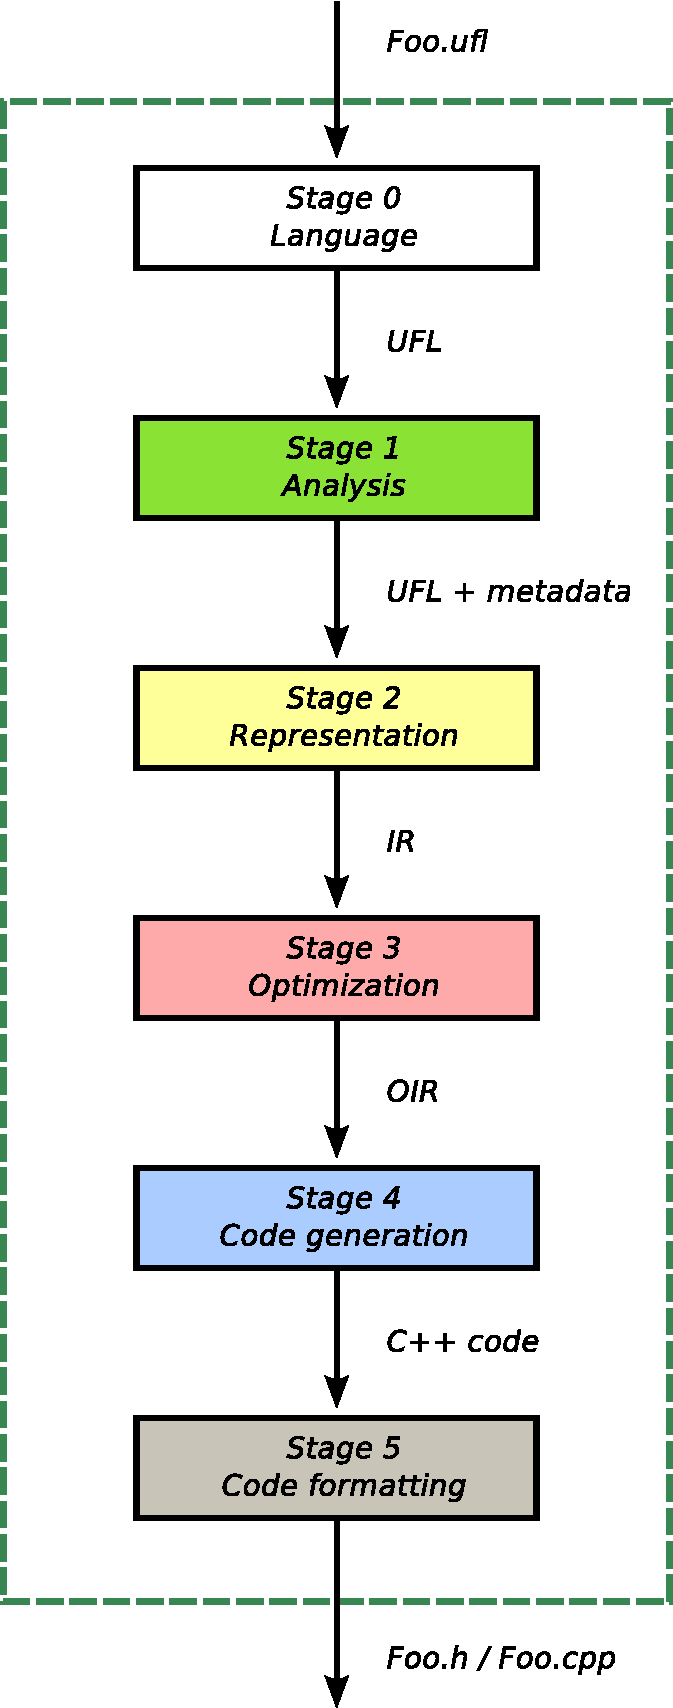
\includegraphics[height=0.8\textheight]{chapters/logg-1/pdf/compilerdesign.pdf}
    \caption{Form compilation broken into six sequential stages:
      Language, Analysis, Representation, Optimization, Code
      generation and Code Formatting. Each stage generates output
      based on input from the previous stage. The input/output data
      consist of a UFL form file (in the case of calling FFC from the
      command-line), a UFL object, a UFL object and metadata computed
      from the UFL object, an intermediate representation (IR), an
      optimized intermediate representation (OIR), C++ code and,
      finally, C++ code files.}
    \label{fig:logg-1:compilerstages}
  \end{center}
\end{figure}

\begin{description}
\item[Compiler stage 0: Language (parsing).]
  In this stage, the user-specified form is interpreted and stored as a
  UFL abstract syntax tree (AST). The actual parsing is handled by
  Python and the transformation to a UFL form object is implemented by
  operator overloading in UFL. \\*[1ex]
  \begin{tabular}{ll}
    \emph{Input:}  & Python code or \emp{.ufl} file \\
    \emph{Output:} & UFL form
  \end{tabular}
  %
\item[Compiler stage 1: Analysis.]
  This stage preprocesses the UFL form and extracts form meta data
  (\emp{FormData}), such as which elements were used to define the form,
  the number of coefficients and the cell type (intervals, triangles,
  or tetrahedra). This stage also involves selecting a suitable
  representation for the form if that has not been specified by the user
  (see Section~\ref{sec:logg-1:representation} below). \\*[1ex]
  %
  \begin{tabular}{ll}
    \emph{Input:}  & UFL form \\
    \emph{Output:} & preprocessed UFL form and form meta data
  \end{tabular}
  %
\item[Compiler stage 2: Code representation.]
  This stage examines the input and generates all data needed for the
  code generation. This includes generation of finite element basis
  functions, extraction of data for mapping of degrees of freedom, and
  possible precomputation of integrals. Most of the complexity of
  compilation is handled in this stage.

  The intermediate representation is stored as a dictionary, mapping
  names of UFC functions to the data needed for generation of the
  corresponding code. In simple cases, like \emp{ufc::form::rank},
  this data may be a simple number like~\emp{2}. In other cases,
  like \emp{ufc::cell\_tensor::tabulate\_tensor}, the data may be a
  complex data structure that depends on the choice of form
  representation. \\*[1ex]
  %
  \begin{tabular}{ll}
    \emph{Input:}  & preprocessed UFL form and form meta data \\
    \emph{Output:} & intermediate representation (IR)
  \end{tabular}
  %
\item[Compiler stage 3: Optimization.]
  This stage examines the intermediate representation and performs
  optimizations. Such optimization may involve FErari based
  optimizations as discussed in Chapter~\ref{chap:kirby-3} or symbolic
  optimization as discussed in Chapter~\ref{chap:oelgaard-2}.
  Data stored in the
  intermediate representation dictionary is then replaced by new data
  that encode an optimized version of the function in question. \\*[1ex]
  %
  \begin{tabular}{ll}
    \emph{Input:}  & intermediate representation (IR) \\
    \emph{Output:} & optimized intermediate representation (OIR)
  \end{tabular}
  %
\item[Compiler stage 4: Code generation.]
  This stage examines the optimized intermediate representation and
  generates the actual C++ code for the body of each UFC function. The
  code is stored as a dictionary, mapping names of UFC functions to
  strings containing the C++ code. As an example, the data generated for
  \emp{ufc::form::rank} may be the string ``\emp{return~2;}''.

  We emphasize the importance of separating stages 2, 3 and 4. This
  allows stages~2 and 3 to focus on algorithmic aspects related to finite
  elements and variational forms, while stage~4 is concerned only with
  generating C++ code from a set of instructions prepared in earlier
  compilation stages. \\*[1ex]
  %
  \begin{tabular}{ll}
    \emph{Input:}  & optimized intermediate representation (OIR) \\
    \emph{Output:} & C++ code
  \end{tabular}
  %
\item[Compiler stage 5: Code formatting.]
  This stage examines the generated C++ code and formats it according to
  the UFC format, generating as output one or more \emp{.h}/\emp{.cpp} files
  conforming to the UFC specification. This is where the actual writing of C++
  code takes place. This stage relies on templates for UFC code
  available as part of the UFC module \emp{ufc\_utils}. \\*[1ex]
  %
  \begin{tabular}{ll}
    \emph{Input:}  & C++ code \\
    \emph{Output:} & C++ code files
  \end{tabular}
\end{description}

%------------------------------------------------------------------------------
\section{Form representation}
\label{sec:logg-1:representation}
\index{form representation}

Two different approaches to code generation are implemented in
FFC. One based on traditional quadrature and another on a special
tensor representation. We address these representations here briefly
and refer readers to Chapter~\ref{chap:oelgaard-2} for details of the quadrature
representation and to Chapter~\ref{chap:kirby-8} for details of the tensor
representation.

%------------------------------------------------------------------------------
\subsection{Quadrature representation}
\index{quadrature representation}

The quadrature representation in \ffc{} is selected using the
option \emp{-r quadrature}.  As the name suggests, the method to
evaluate the local element tensor $A_T$ involves a loop over
integration points and adding the contribution from each point to
$A_T$. To generate code for quadrature, FFC calls FIAT during code
generation to tabulate finite element basis functions and their
derivatives at a suitable set of quadrature points on the reference
element. It then goes on to generate code for computing a weighted
average of the integrand defined by the UFL AST at these quadrature
points.

%------------------------------------------------------------------------------
\subsection{Tensor representation}
\index{tensor representation}

When FFC is called with the \emp{-r tensor} option,
it attempts to extract a monomial representation of the given UFL
form; that is, rewrite the given form as a sum of products of basis
functions and their derivatives. Such a representation is not always
possible, in particular if the form is expressed using operators other
than addition, multiplication and linear differential operators. If
unsuccessful, FFC falls back to using quadrature representation.

If the transformation is successful, FFC computes the tensor
representation $A_T = A^0 : G_T$, as described in Chapter~\ref{chap:kirby-8},
by calling FIAT to compute the reference tensor~$A^0$. Code is then
generated for computing the element tensor. Each entry of the element
tensor is obtained by computing an inner product between the geometry
tensor $G_T$ and a particular slice of the reference tensor. It should
be noted that the entries of the reference tensor are known during
code generation, so these numbers enter directly into the generated
code.

%------------------------------------------------------------------------------
\subsection{Automatic selection of representation}

If the user does not specify which representation to use, \ffc{} will
try to automatically select the ``best'' representation; that is, the
representation that is believed to yield the best run-time
performance. As described in Chapter~\ref{chap:oelgaard-2}, the
run-time performance depends on many factors and it might not be
possible to give a precise \apriori{} answer as to which
representation will be best for a particular variational form. In
general, the more complex the form (in terms of the number of
derivatives and the number of function products), the more likely
quadrature is to be preferable. See \citet{OelgaardWells2010} for a
detailed discussion on form complexity and comparisons between tensor
and quadrature representations. In \citet{OelgaardWells2010}, it was
suggested that the selection should be based on an estimate of the
operation count to compute the element tensor~$A_T$.  However, it
turns out to be difficult to obtain an estimate which is accurate
enough for this purpose. Therefore, the following crude strategy to
select the representation has been implemented. First, \ffc{} will try
to generate the tensor representation and in case it fails, quadrature
representation will be selected. If the tensor representation is
generated successfully, each monomial is investigated and if the
number of coefficients plus derivatives is greater than three, then
quadrature representation is selected for the given variational form.

%------------------------------------------------------------------------------
\section{Optimization}
\index{optimization}

The optimization stage of \ffc{} is concerned with the run-time
efficiency of the generated code for computing the local finite
element tensor. Optimization is available for both quadrature and
tensor representations, and they both operate on the intermediate
representation generated in stage two. The output in both cases is a
new set of instructions (an optimized intermediate representation) for
the code generation stage. The goal of the optimization is to reduce
the number of operations needed to compute the element tensor~$A_T$.

Due to the dissimilar nature of the quadrature and tensor representations,
the optimizations applied to the two representations are different.
To optimize the tensor representation, \ffc{} relies on the Python
module \ferari{} (see Chapter~\ref{chap:kirby-3}) to perform the
optimizations. Optimization strategies for the quadrature representation
are implemented as part of the \ffc{} module itself and are described
in~Chapter~\ref{chap:oelgaard-2}.  For both representations, the
optimizations come at the expense of an increased generation time for
\ffc{} and for very complicated variational forms, hardware limitations
can make the compilation impossible.

Optimizations are switched on by using the command-line
option \emp{-O} or through the Python interface by setting the
parameter \emp{optimize} equal to \emp{True}. For the quadrature
representation, there exist four optimization strategy options,
and these can be selected through the command-line interface by giving
the additional options \emp{-f eliminate\_zeros}, \emp{-f
simplify\_expressions},
\emp{-f precompute\_ip\_const} and \emp{-f precompute\_basis\_const},
and through the Python interface by setting these
parameters equal to \emp{True} in the options dictionary.
The option \emp{-f eliminate\_zeros} can be combined with
any of the other three options.
Only one of the optimizations \emp{-f simplify\_expressions},
\emp{-f precompute\_ip\_const} and \emp{-f precompute\_basis\_const} can be
switched on at one time, and if two are given \emp{-f simplify\_expressions}
takes precedence over \emp{-f precompute\_ip\_const} which in turn takes
precedence over the option \emp{-f precompute\_basis\_const}.
If no specific optimization options are given; that is,
only \emp{-O} is specified, the default is to switch on the
optimizations \emp{-f eliminate\_zeros} and
\emp{-f simplify\_expressions}.

%------------------------------------------------------------------------------
\section{Just-in-time compilation}
\label{sec:logg-1:jit}
\index{just-in-time compilation}
\index{JIT compilation}

\ffc{} can also be used as a just-in-time (JIT) compiler. In a scripted
environment, \ufl{} objects can be passed to \ffc{}, and \ffc{} will
return Python modules. Calling the JIT compiler involves calling the
\emp{jit} function available as part of the FFC Python module:
%
\begin{python}
(compiled_object, compiled_module, form_data, prefix) \
    = jit(ufl_object, parameters=None, common_cell=None)
\end{python}
where \emp{ufl\_object} is either a \ufl{} form or finite element
object, \emp{parameters} is an optional dictionary containing form
compiler parameters and \emp{common\_cell} is an optional argument.
The \emp{common\_cell} argument may be used to specify the cell
(interval, triangle or tetrahedron) when the cell is not specified as
part of the form\footnote{This is used by DOLFIN to allow simple
  specification of expressions such as \emp{f =
    Expression("sin(x[0])")} where the choice of cell type is not
  specified as part of the expression.}. The \emp{jit} function
returns a tuple, where \emp{compiled\_form} is a Python object which
wraps either \emp{ufc::form} or \emp{ufc::finite\_element} (depending
on the type of \ufl{} object passed to the form compiler),
\emp{compiled\_module} is a Python module which wraps all the
generated \ufc{} code (this includes finite elements, degree of
freedom maps, etc.), \emp{form\_data} is a \ufl{} object that contains
form metadata such as the number of coefficient functions in a form,
and \emp{prefix} is a string identifier for the form.

When the JIT compiler is called, internally \ffc{} generates \ufc{}
code for the given form or finite element, compiles the generated code
using a C++ compiler, and then wraps the result as a Python module using
SWIG and Instant (see Chapter~\ref{chap:wilbers}).  The returned objects
are ready to be used from Python.  The generated and wrapped code is
cached by the JIT compiler, so if the JIT compiler is called twice
for the same form or finite element, the cached version is used. The
cache directory is created by Instant, and can be cleaned by running the
command \emp{instant-clean}.  The interactions of various components in
the JIT process are illustrated in Figure~\ref{fig:logg-1:jit}.

The Python interface of \dolfin{} makes extensive use of JIT
compilation. It makes it possible to combine the performance features
of generated C++ code with the ease of a scripted interface.

\begin{figure}
  \begin{center}
    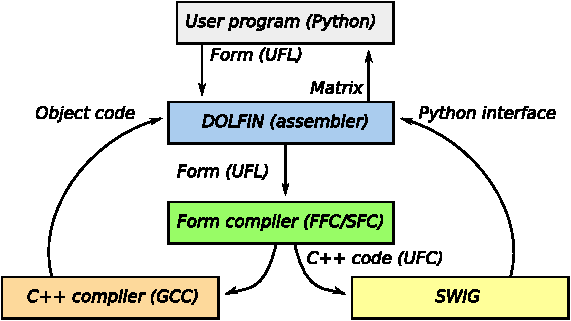
\includegraphics[width=10cm]{chapters/logg-1/pdf/jit.pdf}
    \caption{JIT compilation of variational forms coordinated by
      DOLFIN, and relying on UFL, FFC, UFL, SWIG, and GCC.}
    \label{fig:logg-1:jit}
  \end{center}
\end{figure}

%------------------------------------------------------------------------------
\section{Extending FFC}

FFC may be extended to add support for other languages, architectures
and code generation techniques. For code that conforms to the UFC
interface specification, only compiler stage~4 is affected. In this
stage, the compiler needs to translate the intermediate representation
of the form into actual C++ code that will later be formatted as part
of UFC C++ classes and functions. Possible extensions in this stage of
the compilation process can be to replace loops by special-purpose
library calls (like low-level BLAS calls), SSE instructions or code
targeted for graphical processing units (GPU).

Functionality that requires extending the UFC interface is usually
handled by adding new experimental virtual (but non-abstract)
functions\footnote{The functions are made virtual, but non-abstract to
  ensure backwards compatibility with old generated code.} to the UFC
interface, which may later be proposed to be included in the next
stable specification of the UFC interface. Extensions to other
languages are also possible by replacing the UFC code generation
templates.

%------------------------------------------------------------------------------
\section{Historical notes}

FFC was first released in 2004 as a research code capable of
generating C++ code for simple variational forms
\citep{KirbyLogg2006,KirbyLogg2007}. Ever since its first release,
FFC has relied on FIAT as a backend for computing finite element basis
functions. In 2005, the DOLFIN assembler was redesigned to rely on
code generated by FFC at compile-time for evaluation of the element
tensor. Earlier versions of DOLFIN were based on a run-time system for
evaluation of variational forms in C++ via operator overloading, see
Figures~\ref{fig:logg-1:poisson,before}--\ref{fig:logg-1:poisson,ufl}.

\begin{figure}
  \begin{center}
\begin{c++}
class Poisson : public PDE
{
public:

  Poisson(Function& source) : PDE(3)
  {
    add(f, source);
  }

  real lhs(const ShapeFunction& u,
           const ShapeFunction& v)
  {
    return (grad(u), grad(v))*dx;
  }

  real rhs(const ShapeFunction& v)
  {
    return f*v*dx;
  }

private:

  ElementFunction f;

};
\end{c++}
  \caption{Implementation of Poisson's equation in DOLFIN~0.5.2 using C++ operator overloading.
           Note the use of \texttt{operator,} for inner product.}
  \label{fig:logg-1:poisson,before}
  \end{center}
\end{figure}

\begin{figure}
  \begin{center}
\begin{python}
name = "Poisson"
element = FiniteElement("Lagrange", "triangle", 1)

v = BasisFunction(element)
u = BasisFunction(element)
f = Function(element)

a = v.dx(i)*u.dx(i)*dx
L = v*f*dx
\end{python}
\caption{Implementation of Poisson's equation in DOLFIN~0.5.3 using
  the new FFC form language. Note that the \texttt{grad} operator
  was missing in FFC at this time. It was also at this time that the
  test and trial functions changed places.}
\label{fig:logg-1:poisson,after}
  \end{center}
\end{figure}

\begin{figure}
  \begin{center}
\begin{uflcode}
element = FiniteElement("Lagrange", triangle, 1)

u = TrialFunction(element)
v = TestFunction(element)
f = Coefficient(element)

a = inner(grad(u), grad(v))*dx
L = f*v*dx
\end{uflcode}
\caption{Implementation of Poisson's equation in DOLFIN~1.0 using
  the new UFL form language which was introduced in FFC~0.6.2. The
  order of trial and test functions has been restored.}
\label{fig:logg-1:poisson,ufl}
  \end{center}
\end{figure}

Important milestones in the development of FFC include support for
mixed elements (2005), FErari-based optimizations (2006), JIT
compilation (2007), discontinuous Galerkin methods (2007)
\citep{OelgaardLoggWells2008}, $H(\mathrm{div})/H(\mathrm{curl})$
elements (2007--2008) \citep{RognesKirbyLogg2009}, code generation
based on quadrature (2007) \citep{OelgaardWells2010}, the introduction
of the UFC interface (2007), and optimized quadrature code generation
(2008). In 2009, the FFC form language was replaced by the new UFL
form language.
